\thispagestyle{lichsutoanhocnone}
\pagestyle{lichsutoanhoc}
\graphicspath{{../lichsutoanhoc/pic/}}
\everymath{\color{lichsutoanhoc}}
%\blfootnote{$^1$\color{lichsutoanhoc}Hà Nội.}
\begingroup
\AddToShipoutPicture*{\put(0,616){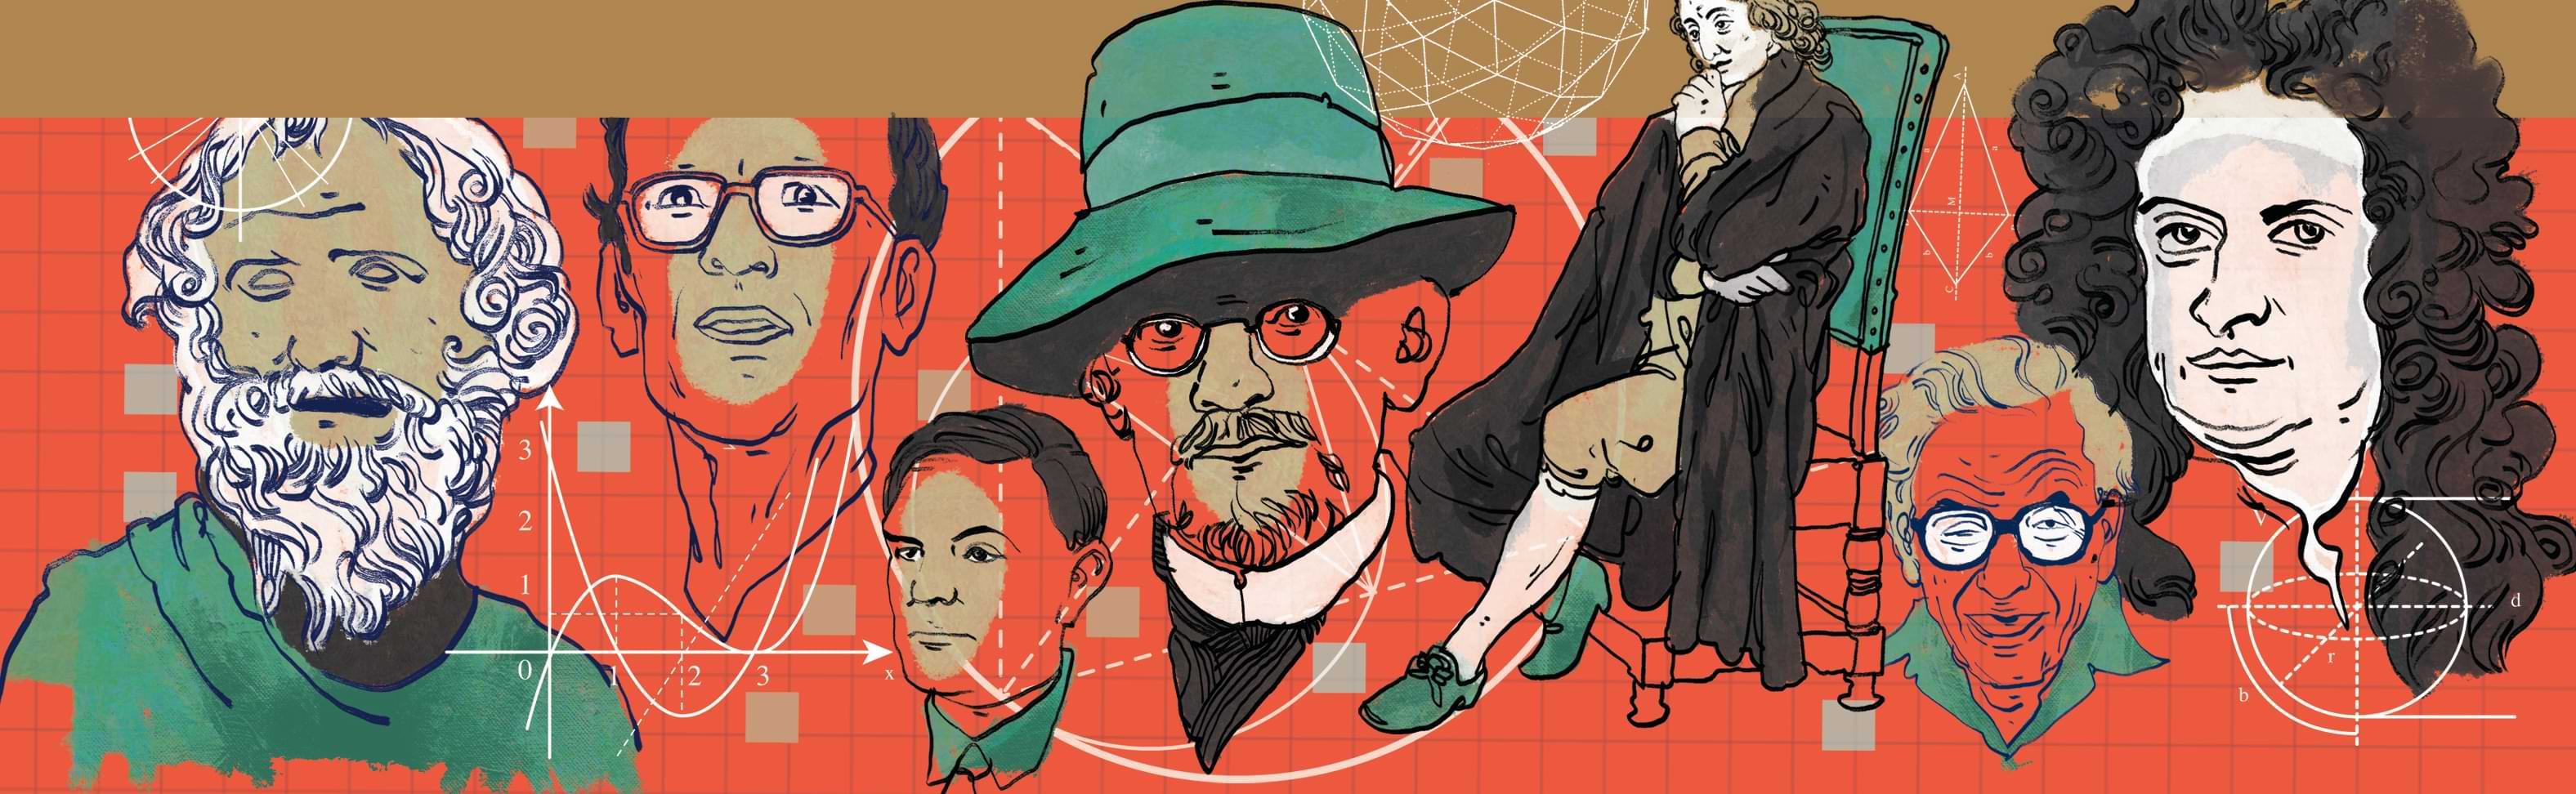
\includegraphics[width=19.3cm]{../bannerlichsu}}}
\AddToShipoutPicture*{\put(62,517){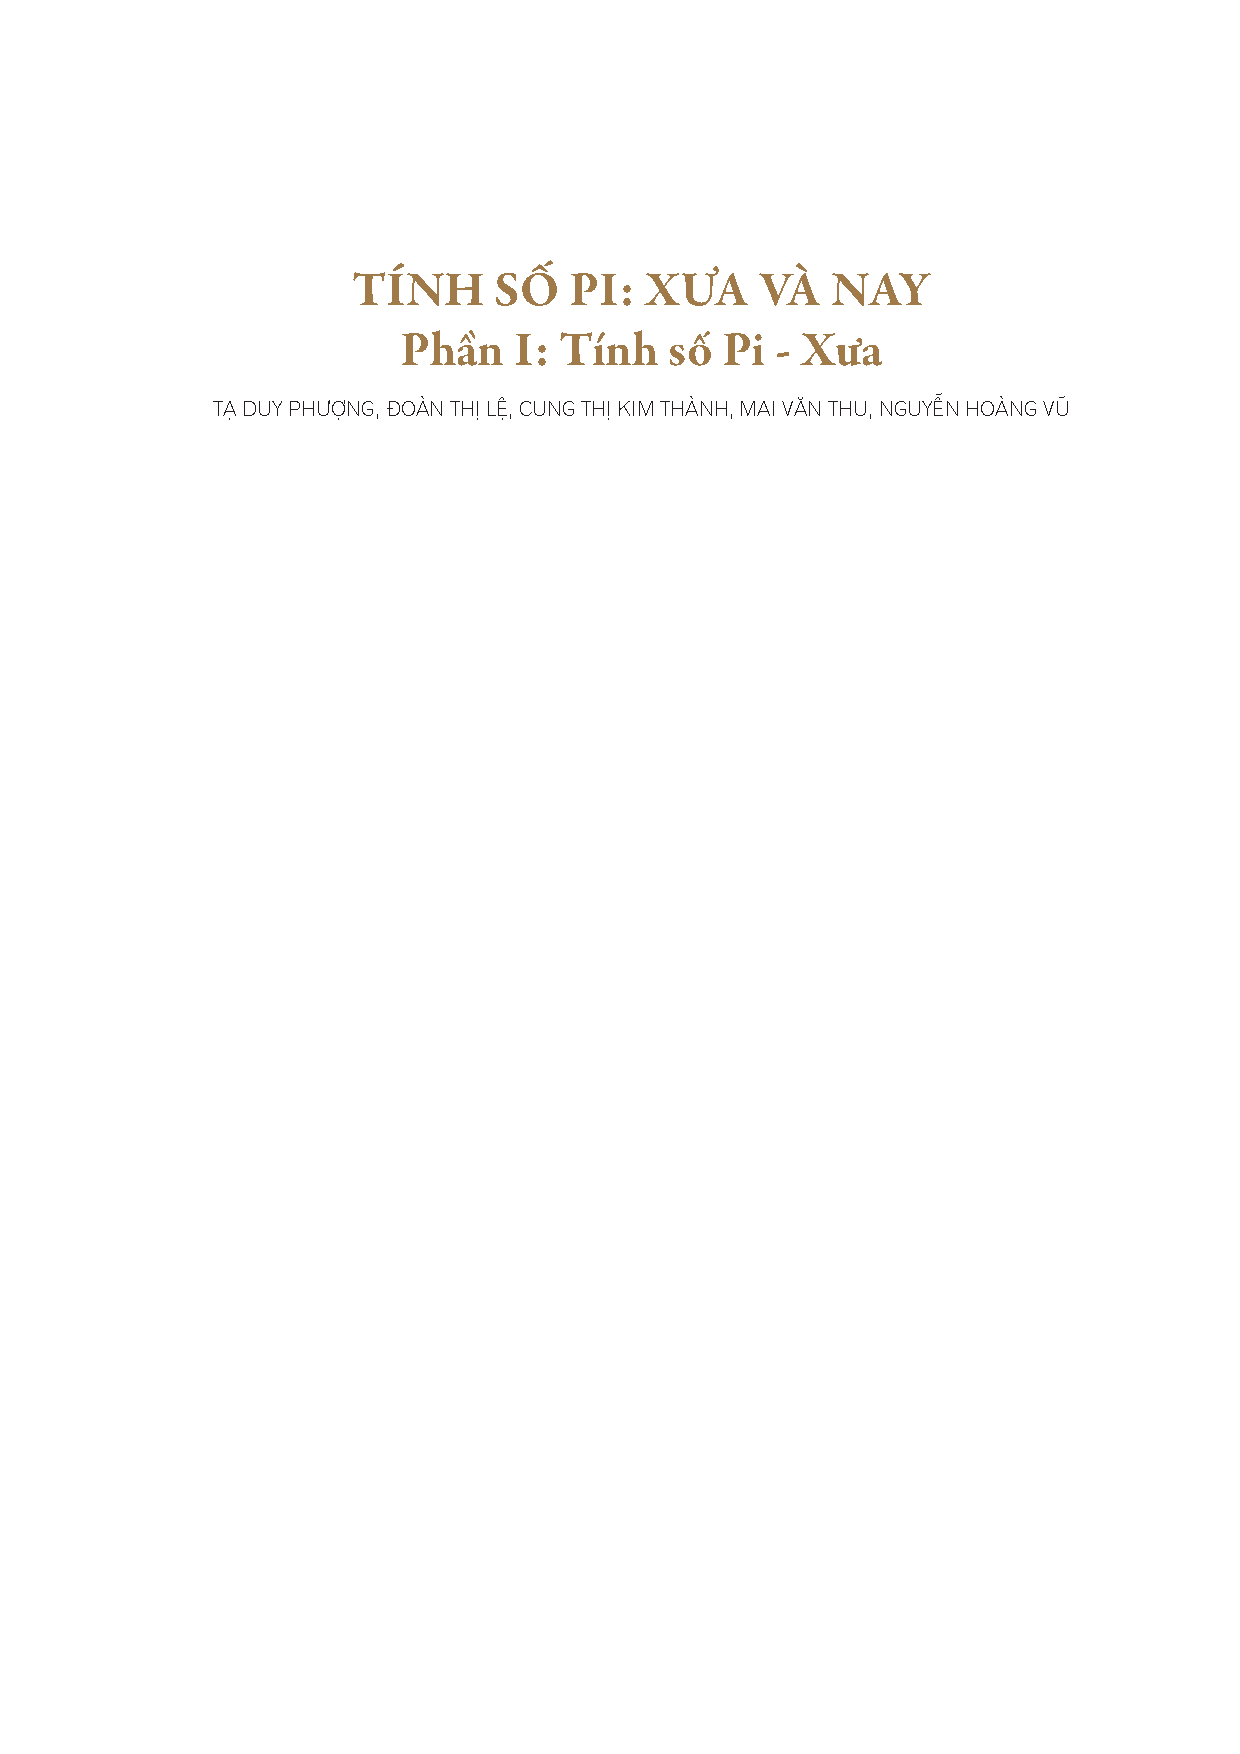
\includegraphics[scale=1]{../tieude.pdf}}}
\centering
\endgroup

\vspace*{185pt}

\begin{multicols}{2}
	Một số vô tỷ rất quen thuộc và có nhiều ý nghĩa thực tế là tỷ số giữa chu vi đường tròn và đường kính của nó, lần đầu tiên được nhà toán học Anh William Jones ($1675-1749$) ký hiệu bằng chữ $\pi$ vào năm $1706$  trong cuốn sách \textit{Synopsis Palmariorum Matheseos} (\textit{Nhập môn Toán học mới}). Chữ $\pi$ là chữ cái đầu tiên trong chữ Hy Lạp \textit{περιφέρεια} (\textit{periphery--viền ngoài, chu vi}). Năm $1748$, trong cuốn sách rất phổ biến, \textit{Introductio in analysin infinitorum} (\textit{Nhập môn Giải tích vô hạn}), Euler viết: ``\textit{để ngắn gọn, ta sẽ ký hiệu $\pi$ bằng một nửa chu vi của đường tròn bán kính bằng $1$}". Từ đó $\pi$ được phổ biến ở châu Âu và ngày nay đã trở thành ký hiệu toán học quen thuộc với tất cả mọi người.
	\vskip 0.1cm
	\textbf{\color{lichsutoanhoc}Số Pi trước toán học Hy Lạp}
	\vskip 0.1cm
	Người Babylon (khoảng $1800-1600$ trước Công nguyên) tính chu vi một đường tròn bằng ba lần đường kính của nó. Hơn nữa, họ còn chính xác hơn khi chọn diện tích hình tròn theo công thức $S = \dfrac{2}{{25}}{L^2},$  trong đó $L$  là chu vi hình tròn. Như vậy, so với công thức chính xác $S = \pi {R^2} = \dfrac{1}{{4\pi }}{\left( {2\pi R} \right)^2}$  thì số  khá chính xác với $\pi  \approx 3{,}1416$.
	\vskip 0.1cm
	Bài toán $48$ trong bản giấy cói Ahmes (Ahmes Rhind Papyrus, $1850$ trước Công nguyên) phát biểu như sau. \textit{Đường tròn có đường kính $9$ khet} (đơn vị độ dài). \textit{Diện tích của nó là bao nhiêu?}
	\vskip 0.1cm
	\textit{Giải:} Bỏ đi $\dfrac{1}{9}$ trong đường kính, cụ thể là $1$, còn $8$. Nhân $8$ với $8$, diện tích của nó là $64$.
	\vskip 0.1cm 
	Bài toán này cho thấy, người Ai Cập cổ đại đã tính diện tích  $S$ của hình tròn có đường kính $d$ bằng diện tích hình vuông có cạnh bằng $\dfrac{8}{9}d$: 
	\setlength{\abovedisplayskip}{5pt}
	\setlength{\belowdisplayskip}{5pt}
	\begin{align*}
		S = {\left( {d - \dfrac{1}{9}d} \right)^2} = {\left( {\dfrac{8}{9}d} \right)^2} = \dfrac{{64}}{{81}}{d^2}.
	\end{align*}
	Từ đây ta có  $S = \dfrac{{64}}{{81}}{d^2} \approx  \pi \dfrac{{{d^2}}}{4}$. Suy ra
	\begin{align*}
		\pi  \approx  \dfrac{{64 \times 4}}{{81}} = \dfrac{{256}}{{81}} \approx 3{,}16049.
	\end{align*}
	Sai số của số này so với  $\pi  \approx 3{,}14156$ là gần $2\%$ và có phân số xấp xỉ là $3\dfrac{1}{7} = \dfrac{{22}}{7} \approx 3{,}14286$.
	\vskip 0.1cm 
	Giả sử cắt ở bốn góc của hình vuông cạnh $9$ \textit{khet} (đơn vị dài) bốn tam giác vuông cân có cạnh bằng $3$ \textit{khet}. Khi ấy diện tích bát giác còn lại gần bằng diện tích hình tròn (hình tròn có phần nằm trong, cũng có phần nằm ngoài bát giác, Hình $1$). Ta có ${S_{{\text{bát giác}}}} = {9^2} - 4.\dfrac{{{3^2}}}{2} = 63.$   
	Giá trị này gần với giá trị  $S = {\left( {\dfrac{8}{9}d} \right)^2} = 64$ khi cho $d = 9$, là cơ sở để giải thích công thức tính diện tích hình tròn $S = \dfrac{{64}}{{81}}{d^2}$  của người Babylon.	 
	\begin{figure}[H]
		\vspace*{-5pt}
		\centering
		\captionsetup{labelformat= empty, justification=centering}
		\begin{tikzpicture}[lichsutoanhoc, scale=0.6]
			\draw  (0.,0.) circle (3.cm);
			\draw  (-3.,-3.)-- (3.,-3.);
			\draw  (3.,-3.)-- (3.,3.);
			\draw  (3.,3.)-- (-3.,3.);
			\draw  (-3.,3.)-- (-3.,-3.);
			\draw  (1.,3.)-- (3.,1.);
			\draw  (3.,-1.)-- (1.,-3.);
			\draw  (-1.,-3.)-- (-3.,-1.);
			\draw  (-3.,1.)-- (-1.,3.);
				\draw [fill=white] (3.,0.) circle (1.5pt);
				\draw [fill=white] (-3.,-3.) circle (1.5pt);
				\draw [fill=white] (3.,-3.) circle (1.5pt);
				\draw [fill=white] (3.,3.) circle (1.5pt);
				\draw [fill=white] (-3.,3.) circle (1.5pt);
				\draw [fill=white] (1.,3.) circle (1.5pt);
				\draw [fill=white] (3.,1.) circle (1.5pt);
				\draw [fill=white] (3.,-1.) circle (1.5pt);
				\draw [fill=white] (1.,-3.) circle (1.5pt);
				\draw [fill=white] (-1.,-3.) circle (1.5pt);
				\draw [fill=white] (-3.,-1.) circle (1.5pt);
				\draw [fill=white] (-3.,1.) circle (1.5pt);
				\draw [fill=white] (-1.,3.) circle (1.5pt);
		\end{tikzpicture}
		\caption{\small\textit{\color{lichsutoanhoc}Hình $1$.}}
		\vspace*{-10pt}
	\end{figure}
	Trong bài toán khắc trên bảng đồng của người Babylon, số $\pi$  được chọn bằng $\dfrac{{25}}{8} = 3{,}125$.
	\vskip 0.1cm   
	Khi đo đạc Đại kim tự tháp Giza ($2500$ trước Công nguyên), các nhà khảo cổ học đã nhận thấy người Ai Cập chọn số $\pi$  bằng $\dfrac{{22}}{7} \approx 3{,}14$.
	\vskip 0.1cm   
	Người  Do Thái cũng lấy $\pi = 3$.  Điều này được thấy trong kinh Cựu Ước, khi nói về bồn tắm tròn trong lâu đài của nhà vua Salomon. 
	\vskip 0.1cm
	\textbf{\color{lichsutoanhoc}Số Pi trong toán học Hy Lạp}
	\vskip 0.1cm
	Thuật toán đầu tiên tính gần đúng số $\pi$  được nhà toán học Hy Lạp Archimedes (khoảng $287-212$ trước Công nguyên) trình bày trong cuốn sách  \textit{Measurement of the Circle} (\textit{Đo hình tròn}). Ông  đã tính được 
	\begin{align*}
		3\dfrac{{10}}{{71}} < \pi  < 3\dfrac{{10}}{{70}} \tag{$1$}
	\end{align*}
	bằng cách xét các đa giác đều $96$ cạnh nội tiếp và ngoại tiếp đường tròn như sau. 
	\vskip 0.1cm
	Giả sử $p_n$  và  $P_n$ là chu vi các đa giác đều $n$  cạnh nội tiếp và ngoại tiếp đường tròn chu vi $C$.  Khi ấy ta có 
	\begin{align*}
		{p_6} &< {p_{12}} < {p_{24}} < {p_{48}} < {\rm{ }}{p_{96}} < ... < {p_n} \\
		&< ... < C < ... < {P_n} < ... < {P_{96}} < {P_{48}} \\
		&< {P_{24}} < {P_{12}} < {P_6}.
	\end{align*}
	Dãy số $\{p_n\}$  là dãy số tăng, bị chặn trên bởi $C$  và $\{P_n\}$  là dãy số giảm bị chặn dưới bởi $C$.  Do đó chúng có giới hạn và có thể chứng minh giới hạn chung của chúng là  $C$.
	\vskip 0.1cm
	Giả sử  $Z$ là tâm hình tròn, và $AB = 2t$  và $CD = 2s$   tương ứng là độ dài một cạnh của các đa giác đều $n$  cạnh ngoại tiếp và nội tiếp hình tròn. Gọi $M$  là điểm giữa của $AB$, $N$ là điểm giữa của  $CD$ và $O$  là giao điểm của tiếp tuyến tại điểm  $C$ với $MA$  (Hình $2$). Tương ứng $OM = OC = t'$  là nửa cạnh của đa giác đều $2n$  cạnh ngoại tiếp và $MC = MD = 2s'$ là cạnh của đa giác đều $2n$ cạnh nội tiếp đường tròn.     
	\begin{figure}[H]
		\vspace*{-5pt}
		\centering
		\captionsetup{labelformat= empty, justification=centering}
		\begin{tikzpicture}[lichsutoanhoc,scale=1.3,node font= \small]
			\draw  (-1.414213562373095,-1.4142135623730954)-- (1.414213562373095,-1.414213562373095);
			\draw [shift={(0.,0.)},]  plot[domain=3.9269908169872414:5.497787143782138,variable=\t]({1.*2.*cos(\t r)+0.*2.*sin(\t r)},{0.*2.*cos(\t r)+1.*2.*sin(\t r)});
			\draw  (0.,0.)-- (-2.,-2.);
			\draw  (-2.,-2.)-- (2.,-2.);
			\draw  (2.,-2.)-- (0.,0.);
			\draw  (-1.414213562373095,-1.4142135623730954)-- (4.214684851089403E-8,-2.);
			\draw  (4.214684851089403E-8,-2.)-- (1.4142135623730958,-1.414213562373095);
			\draw  (0.8284271247461907,-2.)-- (1.4142135623730958,-1.414213562373095);
			\draw  (0.,0.)-- (4.214684851089403E-8,-2.);
				\draw [fill=white] (-2.,-2.) circle (0.8pt);
				\draw (-2.1070556519764487,-2.185112519201409) node {$B$};
				\draw [fill=white] (2.,-2.) circle (0.8pt);
				\draw (2.0884264234624923,-2.185112519201409) node {$A$};
				\draw [fill=white] (0.,0.) circle (0.8pt);
				\draw (0.01383926033153683,0.19322874030847648) node {$Z$};
				\draw [fill=white] (4.214684851089403E-8,-2.) circle (0.8pt);
				\draw (-0.02320693901008737,-2.1897168707627) node {$M$};
				\draw [fill=white] (0.,-1.4142135623730951) circle (0.8pt);
				\draw (0.15940855934397314,-1.2608345838502717) node {$N$};
				\draw [fill=white] (-1.414213562373095,-1.4142135623730954) circle (0.8pt);
				\draw (-1.5328395621812736,-1.2793576835210838) node {$D$};
				\draw [fill=white] (1.4142135623730958,-1.414213562373095) circle (0.8pt);
				\draw (1.477164134325693,-1.2608345838502717) node {$C$};
				\draw [fill=white] (1.414213562373096,-1.414213562373095) circle (0.8pt);
				\draw [fill=white] (0.8284271247461907,-2.) circle (0.8pt);
				\draw (0.8195940960118633,-2.194374069036815) node {$O$};
		\end{tikzpicture}
		\caption{\small\textit{\color{lichsutoanhoc}Hình $2$.}}
		\vspace*{-10pt}
	\end{figure}
	Vì $ACO$  và $AMZ$ là các tam giác vuông đồng dạng nên  $\dfrac{{t'}}{{t - t'}} = \dfrac{{OC}}{{OA}} = \dfrac{{ZM}}{{ZA}}.$
	\vskip 0.1cm
	Theo Định lý Thales ta có  $\dfrac{s}{t} = \dfrac{{NC}}{{MA}} = \dfrac{{CZ}}{{AZ}}.$
	\vskip 0.1cm
	Vì $MZ = CZ$ nên ta có 
	\begin{align*}
		\dfrac{{t'}}{{t - t'}} = \dfrac{s}{t} \text{\color{black}\,\, hay } t' = \dfrac{{ts}}{{t + s}}.
	\end{align*}
	Vì các tam giác cân $CMD$  và  $COM$ là đồng dạng, nên ta có $\dfrac{{2s'}}{{2s}} = \dfrac{{t'}}{{2s'}},$  nghĩa là  $2{s'^2} = st'.$
	\vskip 0.1cm
	Vì $P_n$  và $p_n$  là chu vi đa giác đều $n$  cạnh, $P_{2n}$  và $p_{2n}$  là chu vi đa giác đều $2n$  cạnh ngoại và nội tiếp hình tròn nên ${p_n} = 2ns,$ ${P_n} = 2nt,$    ${p_{2n}} = 2ns',$   ${P_{2n}} = 2nt'.$
	\vskip 0.1cm
	Vậy $P_{2n}$   là trung bình điều hòa của  $p_n$ và $P_n$:
	\begin{align*}
		{P_{2n}} = 2nt' &= \dfrac{{2nts}}{{t + s}} = \dfrac{{2nt \cdot 2ns}}{{2nt + 2ns}} \\
		&= \dfrac{{{p_n} \cdot {P_n}}}{{{p_n} + {P_n}}}. \tag{$2$}
	\end{align*}
	Và $p_{2n}$ là trung bình nhân của $p_n$  và $P_{2n}$:  
	\begin{align*}
		{p_{2n}} = 2ns' &= 2n\sqrt {s \cdot t'}  = \sqrt {2ns \cdot 2nt'}  \\
		&= \sqrt {{p_n} \cdot {P_{2n}}} . \tag{$3$}
	\end{align*}
	Bắt đầu từ $n = 6$: $p_6 = 3d$ và $P_6 = 2\sqrt{3}d$,  trong đó $d$  là đường kính hình tròn, nhờ các công thức truy hồi ($2$) và ($3$), ta tìm được  $p_{96}$ và  $P_{96}$. Sử dụng đánh giá $\dfrac{{265}}{{153}}{\rm{ }} < \sqrt 3  < \dfrac{{1351}}{{780}}$,  Archimedes tìm được tỷ số giữa chu vi đa giác đều $96$ cạnh và đường kính của hình tròn nội tiếp là 
	\begin{align*}
		14688:4673\dfrac{1}{2} = 3 + \dfrac{{667\dfrac{1}{2}}}{{4673\dfrac{1}{2}}} < 3\dfrac{1}{7} = 3\dfrac{{10}}{{70}}.
	\end{align*}
	Và tỷ số giữa chu vi đa giác đều $96$ cạnh và đường kính của hình tròn ngoại tiếp là
	\begin{align*}
		6336:2077\dfrac{1}{4} > 3\dfrac{{10}}{{71}}.
	\end{align*}
	Vậy ($1$) được chứng minh.
	\vskip 0.1cm
	Ta cũng có thể tính toán cách khác như sau.
	\vskip 0.1cm
	Giả sử đường tròn tâm $O$  có bán kính bằng $1$. $AB$  là một cạnh của hình đa giác đều $n$  cạnh nội tiếp đường tròn, có độ dài là $s_n$. Trong tam giác $OAB,$ kẻ $OC$  vuông góc với $AB$ cắt đường tròn tại  $D$. Suy ra $AD$ và $BD$  là hai cạnh của đa giác đều  $2n$ cạnh, có độ dài là  ${s_{2n}}$  (Hình $3$).
	\begin{figure}[H]
		\vspace*{-10pt}
		\centering
		\captionsetup{labelformat= empty, justification=centering}
		\begin{tikzpicture}[lichsutoanhoc,scale=0.9]
			\draw  (0.,0.) circle (2.cm);
			\draw  (-1.414213562373095,1.4142135623730954)-- (1.4142135623730954,1.4142135623730945);
			\draw  (-1.414213562373095,1.4142135623730954)-- (0.,0.);
			\draw  (0.,0.)-- (1.4142135623730954,1.4142135623730945);
			\draw  (0.,0.)-- (0.,2.);
			\draw  (0.,2.)-- (-1.414213562373095,1.4142135623730954);
			\draw  (0.,2.)-- (1.4142135623730954,1.4142135623730945);
			\draw [fill=white] (0.,0.) circle (1.5pt);
			\draw (0.046257928118391335,-0.21959254276378817) node {$O$};
			\draw [fill=white] (-1.414213562373095,1.4142135623730954) circle (1.5pt);
			\draw (-1.6467653276955618,1.696686527003653) node {$A$};
			\draw [fill=white] (1.4142135623730954,1.4142135623730945) circle (1.5pt);
			\draw (1.5532346723044377,1.7152911781664437) node {$B$};
			\draw [fill=white] (0.,1.414213562373095) circle (1.5pt);
			\draw (0.19509513742071688,1.2873842014222578) node {$C$};
			\draw [fill=white] (0.,2.) circle (1.5pt);
			\draw (-0.00955602536998075,2.3850586200269084) node {$D$};
		\end{tikzpicture}
		\caption{\small\textit{\color{lichsutoanhoc}Hình $3$.}}
		\vspace*{-10pt}
	\end{figure}
	Áp dụng định lý Pythagoras vào tam giác vuông $ACD$  ta có
	\begin{align*}
		A{D^2} = A{C^2} + C{D^2} = A{C^2} + {(OD - OC)^2}.
	\end{align*}
	Lại áp dụng định lý Pythagoras vào tam giác vuông $ACO$  ta được
	\begin{align*}
		OC = \sqrt {O{A^2} - A{C^2}} .
	\end{align*}
	Suy ra 
	\begin{align*}
		A{D^2} = A{C^2} + {\left( {OD - \sqrt {O{A^2} - A{C^2}} } \right)^2}
	\end{align*}
	Với  $OA = OD = 1,\;AC = \dfrac{{{s_n}}}{2},\;AD = {s_{2n}},$ ta có
	\begin{align*}
		&s_{2n}^2 = {\left( {\dfrac{{{s_n}}}{2}} \right)^2} + {\left( {1 - \sqrt {1 - {{\left( {\dfrac{{{s_n}}}{2}} \right)}^2}} } \right)^2}\\
		\implies  &s_{2n}^2 = 2 - \sqrt {4 - s_n^2}.
	\end{align*}
	Suy ra 
	\begin{align*}
		{s_{2n}} = \sqrt {2 - \sqrt {4 - s_n^2} }. \tag{$4$}
	\end{align*}
	Sử dụng công thức ($4$), với hình lục giác đều có cạnh bằng bán kính và bằng $1$ (Hình $4$) ta được 
	\begin{align*}
		{s_{12}} = \sqrt {2 - \sqrt {4 - 1} }  = \sqrt {2 - \sqrt 3 } .
	\end{align*}
	Gấp đôi số cạnh được $n= 12$ thì 
	\begin{align*}
		{s_{24}} &= \sqrt {2 - \sqrt {4 - (2 - \sqrt 3 )} }  \\
		&= \sqrt {2 - \sqrt {2 + \sqrt 3 } } .
	\end{align*}
	Tiếp tục với $n = 24$  thì 
	\begin{align*}
		{s_{48}} = \sqrt {2 - \sqrt {2 + \sqrt {2 + \sqrt 3 } } } .
	\end{align*}
	Và với $n = 96$ thì ta được 
	\begin{align*}
		{s_{96}} = \sqrt {2 - \sqrt {2 + \sqrt {2 + \sqrt {2 + \sqrt 3 } } } } .
	\end{align*}
	\begin{figure}[H]
		\vspace*{-10pt}
		\centering
		\captionsetup{labelformat= empty, justification=centering}
		\begin{tikzpicture}[lichsutoanhoc,scale=0.67]
			\draw  (0.,0.) circle (3.cm);
			\draw  (-1.5,2.5980762113533165)-- (1.5,2.5980762113533165);
			\draw  (1.5,2.5980762113533165)-- (3.,0.);
			\draw  (3.,0.)-- (1.5,-2.5980762113533165);
			\draw  (1.5,-2.5980762113533165)-- (-1.5,-2.5980762113533165);
			\draw  (-1.5,-2.5980762113533165)-- (-3.,0.);
			\draw  (-3.,0.)-- (-1.5,2.5980762113533165);
			\draw  (0.,0.)-- (1.5,2.5980762113533165);
			\draw  (-1.5,2.5980762113533165)-- (0.,0.);
			\draw  (-1.5,2.5980762113533165)-- (0.,3.);
			\draw  (0.,3.)-- (-1.5,2.5980762113533165);
			\draw  (-1.5,2.5980762113533165)-- (-2.598076211353315,1.5);
			\draw  (-2.598076211353315,1.5)-- (-3.,0.);
			\draw  (-3.,0.)-- (-2.5980762113533165,-1.5);
			\draw  (-2.5980762113533165,-1.5)-- (-1.5,-2.5980762113533133);
			\draw  (-1.5,-2.5980762113533133)-- (0.,-3.);
			\draw  (0.,-3.)-- (1.5,-2.598076211353315);
			\draw  (1.5,-2.598076211353315)-- (2.598076211353314,-1.5);
			\draw  (2.598076211353314,-1.5)-- (3.,0.);
			\draw  (3.,0.)-- (2.5980762113533165,1.5);
			\draw  (2.5980762113533165,1.5)-- (1.5,2.5980762113533147);
			\draw  (1.5,2.5980762113533147)-- (0.,3.);
				\draw [fill=white] (0.,0.) circle (1.5pt);
				\draw [fill=white] (3.,0.) circle (1.5pt);
				\draw [fill=white] (-3.,0.) circle (1.5pt);
				\draw [fill=white] (-1.5,-2.5980762113533165) circle (1.5pt);
				\draw [fill=white] (1.5,2.5980762113533165) circle (1.5pt);
				\draw [fill=white] (-1.5,2.5980762113533165) circle (1.5pt);
				\draw [fill=white] (1.5,-2.5980762113533165) circle (1.5pt);
				\draw [fill=white] (0.,3.) circle (1.5pt);
				\draw [fill=white] (-2.598076211353315,1.5) circle (1.5pt);
				\draw [fill=white] (-3.,0.) circle (1.5pt);
				\draw [fill=white] (-2.5980762113533165,-1.5) circle (1.5pt);
				\draw [fill=white] (-1.5,-2.5980762113533133) circle (1.5pt);
				\draw [fill=white] (0.,-3.) circle (1.5pt);
				\draw [fill=white] (1.5,-2.598076211353315) circle (1.5pt);
				\draw [fill=white] (2.598076211353314,-1.5) circle (1.5pt);
				\draw [fill=white] (3.,0.) circle (1.5pt);
				\draw [fill=white] (2.5980762113533165,1.5) circle (1.5pt);
				\draw [fill=white] (1.5,2.5980762113533147) circle (1.5pt);
		\end{tikzpicture}
		\caption{\small\textit{\color{lichsutoanhoc}Hình $4$.}}
		\vspace*{-5pt}
	\end{figure}
	Tỷ số chu vi của đa giác đều $96$ cạnh nội tiếp so với đường kính hình tròn  bằng
	\begin{align*}
		&96\cdot\dfrac{{{s_{96}}}}{2} \\[-1ex]
		= \,\,&48\cdot{s_{96}} = 48\sqrt {2 \!-\! \sqrt {2 \!+\! \sqrt {2 \!+\! \sqrt {2 \!+\! \sqrt 3 } } } }  \\[-0.4ex]
		\approx\,\, &3{,}14103 \approx 3\dfrac{{10}}{{71}}.
	\end{align*}
	Tương tự cho đa giác đều ngoại tiếp, ta có 
	\begin{align*}
		{S_{2n}} = \dfrac{{2\sqrt {4 + S_n^2}  - 4}}{{{S_n}}}. \tag{$5$}
	\end{align*}
	Bắt đầu với một lục giác đều ngoại tiếp một đường tròn (Hình $5$).  Do tam giác  $OAB$ đều nên 
	\begin{align*}
		OA = OB = AB = {S_6};\;\;AC = \dfrac{{{S_6}}}{2};\;\;OC = 1.
	\end{align*}
	Áp dụng định lý Pythagoras cho tam giác vuông $OAC$ ta có
	\begin{align*}
		O{A^2} = O{C^2} + A{C^2} &\implies  S_6^2 = {1^2} + {(\dfrac{{{S_6}}}{2})^2} \\[-0.4ex]
		&\implies {S_6} = \dfrac{{2\sqrt 3 }}{3}.
	\end{align*}
	Theo ($5$) ta sẽ tính được ${S_{12}},{S_{24}},{S_{48}},{S_{96.}}$
	Tỷ số chu vi của đa giác đều $96$ cạnh ngoại tiếp so với đường kính hình tròn  là  
	\begin{align*}
		96.\dfrac{{{S_{96}}}}{2} \approx 3{,}14271 \approx 3\dfrac{{10}}{{70}}.
	\end{align*}
	\begin{figure}[H]
		\vspace*{-10pt}
		\centering
		\captionsetup{labelformat= empty, justification=centering}
		\begin{tikzpicture}[lichsutoanhoc,scale=0.85]
			\draw  (0.,0.) circle (2.cm);
			\draw  (-2.,2.)-- (0.,0.);
			\draw  (0.,0.)-- (2.,2.);
			\draw  (-2.,2.)-- (2.,2.);
			\draw  (0.,2.)-- (0.,0.);
			\draw [fill=white] (0.,0.) circle (1.5pt);
			\draw (0.009048625792809947,-0.20098789160099748) node {$O$};
			\draw [fill=white] (2.,2.) circle (1.5pt);
			\draw (2.129978858350949,2.347849317701327) node {$B$};
			\draw [fill=white] (-2.,2.) circle (1.5pt);
			\draw (-2.093276955602539,2.347849317701327) node {$A$};
			\draw [fill=white] (0.,2.) circle (1.5pt);
			\draw (0.1392811839323448,2.3106400153757454) node {$C$};
		\end{tikzpicture}
		\caption{\small\textit{\color{lichsutoanhoc}Hình $5$.}}
		\vspace*{-10pt}
	\end{figure}
	Vì hình tròn bị giới hạn bởi các đa giác đều nội tiếp và ngoại tiếp, nên ($1$) được chứng minh.
	Trong \textit{Plinthides and Cylinders}, Archimedes còn tính số Pi: 
	\begin{align*}
		\dfrac{{195888}}{{62351}} > \pi  > \dfrac{{211875}}{{67441}}
	\end{align*}
	hay 
	\begin{align*}
		3{,}14697 > \pi  > 3{,}1463911.
	\end{align*}
	Đánh giá này không chính xác vì $\pi  \approx 3{,}141592654$   nằm ngoài khoảng trên. 
	Một đánh giá tinh tế hơn được làm bởi Tannery:
	\begin{align*}
		\dfrac{{195882}}{{62351}} > \pi  > \dfrac{{211872}}{{67441}}
	\end{align*}
	hay 
	\begin{align*}
		3{,}141601578 > \pi  > 3{,}141590427.
	\end{align*}
	Một đánh giá khác là 
	\begin{align*}
		\dfrac{{195888}}{{62351}} > \pi  > \dfrac{{211875}}{{67444}}
	\end{align*}
	hay 
	\begin{align*}
		3{,}141697808 > \pi  > 3{,}141495166.
	\end{align*}
	Khoảng năm $150$ Công nguyên, nhà bác học Ptolemy, trong tác phẩm \textit{Almagest}, dựa trên bảng tính các cung (\textit{Table of Chords}), đã dùng biểu diễn gần đúng số Pi dưới dạng phân số trong hệ đếm cơ số $60$ là 
	\begin{align*}
		\pi  \approx 3 + \dfrac{8}{{60}} + \dfrac{{30}}{{{{60}^2}}} = \dfrac{{377}}{{120}} \approx 3{,}141666667.
	\end{align*}
	Ông cũng nhận xét rằng, số này nằm giữa $3\dfrac{{10}}{{71}}$  và  $3\dfrac{{10}}{{70}}.$
	\vskip 0.1cm
	\textbf{\color{lichsutoanhoc}Số Pi trong toán học Trung Quốc}
	\vskip 0.1cm
	Lúc đầu, người Trung Quốc chấp nhận xấp xỉ $\pi \approx 3$. Đầu thế kỷ II, Trương Hành (張衡, khoảng $78-139$) tìm được  $\pi  \approx \sqrt {10}  \approx 3{,}162$. Bằng cách nội tiếp hình tròn bởi các hình lục giác đều và gấp đôi số cạnh, Lưu Huy  (劉徽, $220-280$) năm $263$ trong cuốn sách Cửu \textit{chương toán thuật} (九章算術) đã tìm được $\pi  \approx 3{,}14$  và sau đó ông tìm được  $\pi  \approx 3{,}14159.$ Tổ Xung Chi (祖沖之, $429-500$), sử dụng thuật toán của Lưu Huy với đa giác $12288 = 3.{2^{12}}$  cạnh, đã tính số $\pi$  chính xác đến $8$ chữ số:
	\begin{align*}
		3{,}1415926 < \;\pi \; < 3{,}1415927\;
	\end{align*}
	Và ông chọn $\pi \; \approx \dfrac{{\;355}}{{113}} \approx 3{,}1415929$
	hoặc  $\pi \; \approx \;\dfrac{{22}}{7} \approx 3{,}145927$. 
	\vskip 0.1cm
	\textbf{\color{lichsutoanhoc}Số Pi trong toán học Việt Nam}
	\vskip 0.1cm
	Lương Thế Vinh ($1441-1497$, [$4$]) và các nhà toán học sau ông, cho đến thế kỉ XVIII, chọn $\pi = 3$.  Nguyễn Hữu Thận ($1757-1831$, [$3$]) đã sử dụng giá trị của số $\pi$ gần đúng đến $8$ chữ số thập phân. Ông đã sử dụng số $\pi  \approx 3{,}14159265$,  trong khi sách \textit{Bút toán chỉ nam} của Nguyễn Cẩn in năm $1909$ [$1$], sau Nguyễn Hữu Thận $80$ năm vẫn dùng số  $\pi$  bằng $3{,}14$ hoặc $3{,}1416$. Tương tự, Phạm Gia Kỉ, trong \textit{Đại thành toán học chỉ minh} [$2$] viết khoảng $1840$ cũng chỉ dùng $\pi$  bằng $3{,}14$ hoặc $3{,}1416$.  Nguyễn Hữu Thận và Nguyễn Cẩn cũng nhắc đến \textit{cách tính của Tây phương} (phương pháp gấp đôi số cạnh của Archimedes). Quan hệ giữa đường kính và chu vi (thông qua số  $\pi$) được Nguyễn Hữu Thận gọi là \textit{định luật chu vi đường kính}. Nguyễn Hữu Thận phát biểu:
	\vskip 0.1cm
	\textbf{\color{lichsutoanhoc}Định luật chu vi đường kính}
	\vskip 0.1cm
	Đường kính $100000000$, chu vi $314159265$
	\vskip 0.1cm
	Lại có chu vi $p = 100000000$, đường kính $d = 31830988$.
	\vskip 0.1cm
	\textit{Giải thích.} Nếu lấy $\pi = 3{,}14159265$, đường kính $d = 100000000$ thì chu vi đường tròn là  $p = d.\pi = 314159265$ (chính xác đến $8$ chữ số).
	\vskip 0.1cm
	Nếu biết chu vi $p = 100000000$,  thì 
	\begin{align*}
		d = \dfrac{p}{\pi } = \dfrac{{1000000}}{{3{,}14159265}} \approx 31830988
	\end{align*}
	(chính xác đến $8$ chữ số).
	\vskip 0.1cm
	Nguyễn Hữu Thận viết: \textit{Phương pháp là cho bên trong hình tròn bao chứa hình vuông, lại từ bên ngoài hình tròn cắt hình vuông. Phép toán đến ức, vạn lần, tập trung tìm sẽ được vô số đầu mối. Trong ngoài đến tập hợp, trong là cạnh huyền chính, ngoài là đường thẳng được cắt. Cho đến vô số đường bao quanh hình tròn, gần giống như trực tuyến mà được số chu vi này, vốn xuất phát từ phép Tây là kỹ lưỡng nhất.}
	\vskip 0.1cm
	\textit{Giải thích}. Đây là phép tính chu vi đường tròn bắt đầu bằng hình vuông nội và ngoại tiếp, sau đó gấp đôi số cạnh (phương pháp của Lưu Huy). 
	Gọi $d$ là đường kính hình tròn, bán kính $r = \dfrac{d}{2}$. Chu vi hình vuông ngoại tiếp bằng $4d > \pi d = 3{,}14$ $d$
	(cạnh hình vuông bằng đường kính). 	
	\begin{figure}[H]
		\vspace*{-5pt}
		\centering
		\captionsetup{labelformat= empty, justification=centering}
		\begin{tikzpicture}[lichsutoanhoc,scale=0.8]
			\draw  (0.,0.) circle (2.cm);
			\draw  (-2.,-2.)-- (2.,-2.);
			\draw  (2.,-2.)-- (2.,2.);
			\draw  (2.,2.)-- (-2.,2.);
			\draw  (-2.,2.)-- (-2.,-2.);
			\draw  (-1.414213562373095,-1.4142135623730954)-- (1.414213562373095,-1.414213562373095);
			\draw  (-1.414213562373095,1.4142135623730954)-- (-1.414213562373095,-1.4142135623730954);
			\draw  (-1.414213562373095,1.4142135623730954)-- (1.4142135623730954,1.4142135623730945);
			\draw  (1.4142135623730954,1.4142135623730945)-- (1.414213562373095,-1.414213562373095);
				\draw [fill=white] (0.,0.) circle (1.5pt);
				\draw [fill=white] (-2.,-2.) circle (1.5pt);
				\draw [fill=white] (2.,-2.) circle (1.5pt);
				\draw [fill=white] (2.,2.) circle (1.5pt);
				\draw [fill=white] (-2.,2.) circle (1.5pt);
				\draw [fill=white] (-1.414213562373095,1.4142135623730954) circle (1.5pt);
				\draw [fill=white] (1.4142135623730954,1.4142135623730945) circle (1.5pt);
				\draw [fill=white] (-1.414213562373095,-1.4142135623730954) circle (1.5pt);
				\draw [fill=white] (1.414213562373095,-1.414213562373095) circle (1.5pt);
		\end{tikzpicture}
		\caption{\small\textit{\color{lichsutoanhoc}Hình $6$.}}
		\vspace*{-10pt}
	\end{figure}
	Hình vuông nội tiếp đường tròn có đường chéo bằng cạnh hình vuông bằng $\dfrac{d}{{\sqrt 2 }} = r\sqrt 2 .$ Do đó  chu vi hình vuông nội tiếp bằng (Hình $6$): $4r\; = 2d\; \approx 2d \times 1{,}4142 \approx 2{,}8284 < d\pi  \approx d.3{,}14 < 4d$.
	Gấp đôi số cạnh đa giác nội ngoại tiếp và tính giới hạn ta được chu vi hình tròn.
	Nguyễn Hữu Thận cũng phát biểu:
	\vskip 0.1cm
	\textbf{\color{lichsutoanhoc}Phép rút gọn chu vi, đường kính}
	\vskip 0.1cm 
	Đường kính: $113$;	Chu vi: $355$
	\vskip 0.1cm
	Suy luận ban đầu là: Phép tính chu vi, đường kính, cách làm tốt dùng đường kính là $7$, đường bao quanh (chu vi) là $22$ thì thừa. Cách tỉ mỉ dùng đường kính là $50$, chu vi là $157$ thì thiếu. Chỉ có sắp đặt đường kính gộp lại là $113$, chu vi là $355$, phù hợp với định luật hơn. Cho nên chọn dùng nó.
	\vskip 0.1cm 
	\textit{Giải thích}. Chu vi hình tròn bằng:
	\begin{align*}
		p = d\pi  &\approx 7 \times 3{,}14159265 \\
		&\approx 21.99114855 < 22;\\
		p = d\pi  &\approx 50 \times 3{,}14159265 \\
		&\approx 157.0796325 > 157.\\
		p=d\pi  &\approx 113 \times 3{,}14159265 \\
		&\approx 354.99996945 < 355.
	\end{align*}
	Sai số:
	\vskip 0.1cm 		
	$1)$ $22 - 21{,}99114855 = 0{,}00885415$;  
	\vskip 0.1cm
	$2)$ $157{,}0796325 - 157 = 0{,}0796325$;
	\vskip 0.1cm
	$3)$ $355 - 354{,}99996 = 0{,}00004$
	($\dfrac{{355}}{{113}}$ chính xác nhất, đến $4$ chữ số).
	\vskip 0.1cm
	Vậy chọn $\pi  \approx \dfrac{{355}}{{113}}$ là phân số chính xác hơn cả. 
	\vskip 0.1cm
	Nguyễn Hữu Thận viết: \textit{Cạnh hình vuông với đường kính hình tròn bằng nhau nhưng diện tích hình vuông và diện tích hình tròn không có cùng định luật.}
	\vskip 0.1cm
	Diện tích hình vuông: $100000000$.
	\vskip 0.1cm	
	Diện tích hình tròn: $78539816$.
	\vskip 0.1cm
	Mặt khác:
	\vskip 0.1cm
	Diện tích hình tròn: $100000000$.
	\vskip 0.1cm 	
	Diện tích hình vuông: $127323954$.
	\vskip 0.1cm
	\textit{Giải thích.} Với cạnh $a = 10000$ thì diện tích hình vuông ${a^2} = 100000000$. Diện tích hình tròn nội tiếp hình vuông có đường kính bằng cạnh hình vuông do đó bằng 
	\setlength{\abovedisplayskip}{7pt}
	\setlength{\belowdisplayskip}{7pt}
	\begin{align*}
			S &= \pi {R^2} = \dfrac{{\pi {d^2}}}{4} = \dfrac{{\pi {a^2}}}{4}\\
			&\approx 3{,}14159265 \times 100000000:4 \\
			&\approx 78539816.	
	\end{align*}
	Nếu diện tích hình tròn là $100000000$ thì diện tích hình vuông là
	\begin{align*}
		{a^2} &= \dfrac{{4S}}{\pi } = \dfrac{{4 \times 100000000}}{{3{,}14159265}}\\ &= 127323954.
	\end{align*}
	Nguyễn Hữu Thận viết:  \textit{Diện tích hình vuông và diện tích hình tròn bằng nhau, cạnh hình vuông và đường kính hình tròn không cùng định luật.}
	\vskip 0.1cm
	Đường kính hình tròn: $100000000$.
	\vskip 0.1cm 
	Cạnh hình vuông: $88622692$.
	\vskip 0.1cm
	Lại có: 
	\vskip 0.1cm
	Cạnh hình vuông: $100000000$.
	\vskip 0.1cm 
	Đường kính hình tròn: $112837916$.
	\vskip 0.1cm
	\textit{Giải thích}. Diện tích hình vuông bằng diện tích hình tròn và bằng 
	\begin{align*}
		S &= \pi {R^2} = \dfrac{{\pi {d^2}}}{4}\\
		&\approx 3{,}14159265 \times {100000000^2}:4 \\
		&\approx 7853981633974483.
	\end{align*}
	Cạnh $a$ của hình vuông bằng
	\begin{align*}
		a = \sqrt S  \approx 88622692.
	\end{align*}
	Tương tự, nếu có cạnh hình vuông bằng $100000000$ thì  
	\begin{align*}
		d &= \sqrt {\dfrac{{4S}}{\pi }}  = \sqrt {\dfrac{{4{a^2}}}{\pi }}  = \dfrac{{2a}}{{\sqrt \pi  }} \\
		&\approx \dfrac{{2 \times 100000000}}{{\sqrt {3{,}14159265} }} \\
		&\approx 112837916.
	\end{align*}
	Như vậy, có thể khẳng định Nguyễn Hữu Thận ($1757-1831$) là người Việt Nam đầu tiên có cảm nhận toán học về số vô tỷ và giới hạn thông qua quan hệ giữa số $\pi$ và diện tích các đa giác đều nội ngoại tiếp hình tròn khi gấp đôi số cạnh.
	\vskip 0.1cm
	\textbf{\color{lichsutoanhoc}Tiếp tục tính gần đúng số Pi}
	\vskip 0.1cm
	Tính toán thiên văn trong \textit{Shatapatha Brahmana} (Ấn Độ, thế kỉ IV trước Công nguyên) dùng xấp xỉ $\pi  \approx \dfrac{{339}}{{108}} \approx \;3{,}139$.  Một số tư liệu cổ của Ấn Độ chọn $\pi  \approx \sqrt {10}  \approx 3{,}162$. Trong tác phẩm \textit{Āryabhaṭīya}, nhà thiên văn Ấn Độ Aryabhata ($476-550$) đã sử dụng giá trị $\pi  = 3{,}1416$.
	\vskip 0.1cm 
	Fibonacci vào năm $1220$ đã tính được $\pi  = 3{,}1418$  độc lập với Archimedes. 
	\vskip 0.1cm
	Tác giả người Ý Dante đã sử dụng giá trị  $\pi  = 3 + \dfrac{{\sqrt 2 }}{{10}} \approx 3{,}14142.$
	\vskip 0.1cm 
	Mãi $8$ thế kỷ sau, kỷ lục của Tổ Xung Chi mới bị phá bởi nhà toán học Ba Tư Al--Kāshānī ($1370-1450$). Ông dùng phương pháp của Archimedes và xét các đa giác đều $3.2^{28}$ cạnh nội tiếp và ngoại tiếp đường tròn và tìm được số $\pi$ đúng tới $17$ chữ số là $3{,}1415926535897932$.  Al--Kāshānī còn dự đoán $\pi$ là số vô tỷ. Điều này chỉ được chứng minh bởi nhà toán học Thụy Sĩ Johann Heinrich Lambert ($1728 - 1777$).
	\vskip 0.1cm 
	Cũng gấp đôi số cạnh như Archimedes, nhưng xuất phát từ hình vuông, nhà toán học Pháp François Viète vào năm $1578$ đã tính chính xác số $\pi$  đến $9$ chữ số nhờ sử dụng đa giác  $3 \times 2^{17}$ cạnh dựa trên công thức
	\begin{align*}
			\dfrac{2}{\pi } = &\cos \dfrac{\pi }{4} \cdot \cos \dfrac{\pi }{8} \cdot \cos \dfrac{\pi }{{16}}...\\
			= &\sqrt {\dfrac{1}{2}}  \cdot \sqrt {\dfrac{1}{2}\left( {1 + \sqrt {\dfrac{1}{2}} } \right)}  \\
			 &\!\times\!\sqrt {\dfrac{1}{2}\left( {1 \!+\! \sqrt {\dfrac{1}{2}\left(\! {1 \!+\! \sqrt {\dfrac{1}{2}} } \!\right)} } \right)} ... \tag{$6$}
	\end{align*}
	\textit{Giải thích}: Sử dụng công thức ${\cos ^2}a = \dfrac{{1 + \cos 2a}}{2}$  và $\cos \dfrac{\pi }{4} = \sqrt {\dfrac{1}{2}},$ ta dễ dàng tính được 
	\begin{align*}
		\cos \dfrac{\pi }{8} &= \sqrt {\dfrac{1}{2}\left( {1 + \sqrt {\dfrac{1}{2}} } \right)};\\
		\cos \dfrac{\pi }{{16}} &= \sqrt {\dfrac{1}{2}\left( {1 + \sqrt {\dfrac{1}{2}\left( {1 + \sqrt {\dfrac{1}{2}} } \right)} } \right)}.
	\end{align*}
	Công lao của François Viète là phát hiện ra công thức biểu diễn ($6$).
	\vskip 0.1cm
	Gọi $A(n)$  là diện tích đa giác đều $n$  cạnh nội tiếp hình tròn bán kính  $r$ và $\beta$ là góc ở tâm.  Ta có (Hình $2$):
	\begin{align*}
		A(n) = n\dfrac{1}{2}{r^2}\sin 2\beta  = n{r^2}\sin \beta \cos \beta .
	\end{align*}
	Tương tự,  
	\begin{align*}
		A(2n) = 2n\dfrac{1}{2}{r^2}\sin \beta  = n{r^2}\sin \beta .
	\end{align*}
	Suy ra
	\begin{align*}
		\dfrac{{A(n)}}{{A(4n)}} = \dfrac{{A(n)}}{{A(2n)}}\cdot\dfrac{{A(2n)}}{{A(4n)}} = \cos \beta \cos \dfrac{\beta }{2}.
	\end{align*}
	Do đó,
	\begin{align*}
			\dfrac{{A(n)}}{{A({2^k}n)}} &= \dfrac{{A(n)}}{{A(2n)}}\cdot\dfrac{{A(2n)}}{{A(4n)}}...\dfrac{{A\left( {{2^{k - 1}}n} \right)}}{{A({2^k}n)}}\\
			&= \cos \beta \cos \dfrac{\beta }{2}...\cos \dfrac{\beta }{{{2^k}}}.
	\end{align*}
	Khi $k$  tiến tới $\infty$  thì $A({2^k}n)$  tiến tới diện tích hình tròn, nghĩa là $\mathop {\lim }\limits_{k \to \infty } A({2^k}n) = \pi {r^2}.$ Suy ra  
	\begin{align*}
		\pi {r^2} &= \dfrac{{A(n)}}{{\cos \beta \cos \dfrac{\beta }{2}...\cos \dfrac{\beta }{{{2^k}}}...}} \\
		&= \dfrac{{\dfrac{1}{2}n{r^2}\sin 2\beta }}{{\cos \beta \cos \dfrac{\beta }{2}...\cos \dfrac{\beta }{{{2^k}}}...}}.
	\end{align*}
	Vậy  
	\begin{align*}
		\pi  = \dfrac{{n\sin 2\beta }}{{2\cos \beta \cos \dfrac{\beta }{2}...\cos \dfrac{\beta }{{{2^k}}}...}}.
	\end{align*}
	Để được công thức ($6$), Viète đã chọn $n = 4$. Khi ấy $\beta  = \dfrac{\pi }{4}$  và 
	\begin{align*}
		\sin 2\beta  = \sin \dfrac{\pi }{2} = 1, \cos \beta  = \cos \dfrac{\pi }{4} = \dfrac{1}{{\sqrt 2 }}.
	\end{align*}
	Nhà toán học Đức Adriaan van Roomen ($1561-1615$) nhận được xấp xỉ số  $\pi$ đến $15$ chữ số vào năm $1593$.
	\vskip 0.1cm 
	Năm $1596$, nhà toán học người Hà Lan Ludolph van Ceulen ($1540-1610$) đã dành $50$ năm trong hơn $70$ năm của đời mình để tính số $\pi$   xấp xỉ đến $35$ chữ số.
	\vskip 0.1cm 
	Năm $1621$, nhà khoa học Đức Willebrord Snellius đã đạt được xấp xỉ số $\pi$  đến $34$ chữ số.
	\vskip 0.1cm
	Năm $1630$, nhà thiên văn người Áo Christoph Grienberger ($1561-1636$) đã tìm được số $\pi$ xấp xỉ đến $38$ chữ số bằng cách sử dụng đa giác đều  $10^{40}$ cạnh.
	\vskip 0.1cm 
	Năm $1654$, Christiaan Huygens đã nhận được xấp xỉ đến $10$ chữ số thập phân nhờ sử dụng phương pháp ngoại suy Richardson.  
	\vskip 0.1cm
	Kỉ lục Christoph Grienberger chỉ bị vượt qua và thuật toán Archimedes đi vào lịch sử khi năm $1699$, số  $\pi$ được tính gần đúng đến $71$ chữ số nhờ phân tích số  $\pi$ dưới dạng chuỗi lũy thừa. Từ đó, số $\pi$ được tính gần đúng nhờ công cụ giải tích. Điều này sẽ được trình bày chi tiết trong Phần $2$.
	\vskip 0.1cm 
	\textbf{\color{lichsutoanhoc}Biểu diễn số $\pmb{\pi}$  dưới dạng phân số liên tục}
	\vskip 0.1cm
	Số $\pi$  có thể biểu diễn dưới dạng phân số liên tục như sau: 
	\begin{align*}
		\pi  \!=\! 3 \!+\! \dfrac{1}{{7 \!+\! \dfrac{1}{{15 \!+\! \dfrac{1}{{1 \!+\! \dfrac{1}{{292 \!+\! \dfrac{1}{{1 \!+\! \dfrac{1}{{1 \!+\! \dfrac{1}{{1 \!+\! ...}}}}}}}}}}}}}}
	\end{align*}
	Cắt cụt phân số này ta lần lượt được  $\pi  \approx 3;$  $\pi  \approx 3 + \dfrac{1}{7} = \dfrac{{22}}{7};$ $\pi  = 3 + \dfrac{1}{{7 + \dfrac{1}{{15}}}} = 3 + \dfrac{{15}}{{106}} = \dfrac{{333}}{{106}};$ $\pi  = 3 + \dfrac{1}{{7 + \dfrac{1}{{15 + 1}}}} = 3 + \dfrac{{16}}{{113}} = \dfrac{{355}}{{113}},$
	là các phân số xấp xỉ số $\pi$ thường gặp trong lịch sử các dân tộc Tây--Đông.
	\vskip 0.1cm
	\textbf{\color{lichsutoanhoc}Thông tin tác giả}
	\vskip 0.1cm
	$\bullet$ Tạ Duy Phượng (PGS Toán học)
	\vskip 0.1cm
	$\bullet$ Đoàn Thị Lệ, Cung Thị Kim Thành (Thạc sĩ Hán Nôm)
	\vskip 0.1cm
	$\bullet$ Mai Văn Thu, Nguyễn Hoàng Vũ (Thạc sĩ Toán học)
	\vskip 0.1cm
	\textbf{\color{lichsutoanhoc}Tài liệu trích dẫn}
	\vskip 0.1cm
	[$1$]   阮菫 Nguyễn Cẩn ($1909$),  \textit{Bút toán chỉ nam}, Thư viện viện nghiên cứu Hán Nôm, Viện nghiên cứu Hán Nôm, VHv. $282$ và A.$1031$. Bản thảo bản dịch của Đoàn Thị Lệ, $2015$.
	\vskip 0.1cm
	[$2$] 范嘉紀  Phạm Gia Kỷ,  大成算學指明  \textit{Đại thành toán học chỉ minh}, Thư viện viện nghiên cứu Hán Nôm, Viện nghiên cứu Hán Nôm, A.$1555$. Bản thảo bản dịch của Phạm Hữu Lộc, $2019$.
	\vskip 0.1cm 
	[$3$]  阮 有 慎 Nguyễn Hữu Thận,  意齋算法一得錄  \textit{Ý Trai toán pháp nhất đắc lục} ($1829$), Thư viện Viện nghiên cứu Hán Nôm, Vhv.$1184$, A.$1336$, A. $982$, A.$1336$/a. Bản thảo bản dịch của Đoàn Thị Lệ và Cung Thị Kim Thành, $2015-2016$.
	\vskip 0.1cm 
	[$4$] 梁世榮  Lương Thế Vinh,  算法大成 \textit{Toán pháp đại thành}, Thư viện Viện nghiên cứu Hán Nôm, Ký hiệu: A.$2931$ và VHv. $1152$. Bản thảo bản dịch của Cung Thị Kim Thành, $2017$.
	\vskip 0.1cm
	[$5$] David M. Burton, \textit{The History of Mathematics, An Introduction}, Seventh Edition, McGraw Hill, $2011$, $819$ p.
	\vskip 0.1cm
	[$6$] Heinrich Dörrie, \textit{The $100$ Great Problems of Elementary Mathematics, Their History and Solution}, New York, Dover Publications, INC., $1965$.
	\vskip 0.1cm     
	[$7$] Thomas Heath, \textit{A History of Greek Mathematics}, Oxford at the Clarendon Press, $1921$, Volume $1$, $232-235$.
	\vskip 0.1cm
	[$8$] Lam Lay--Yong and Ang Tian--Se, Circle Measurements in Ancient China, \textit{Historia Mathematica}, $13$,  ($1986$), $325-340$.
	\vskip 0.1cm
	[$9$] A. Volkov, Calculation of $\pi$ in ancient China: From Liu Hui to Zu Chongzhi, \textit{Historia Scientiarum}, Vol. $4$ ($1994$), No $2$, $139-157$. 
	\vskip 0.1cm
	\hfill (\textit{Còn tiếp})
\end{multicols}